
\subsubsection{Boundary-klasse: Steering}
Denne klasse har til formål at styre bilens retning venstre/højre, hastighed frem/tilbage og bremse bilen. Den får input ind med hastighed frem, hastighed tilbage, retning og brems. Derudover henter klassen den ønskede maksimum hastighed for bilen og den aktuelle hastighed på bilen. Derefter udregner og regulerer den outputtet til PWM for motor. Ligeledes udregner den et PWM output til styretøjs servoen udfra retnings værdien og min/max for duty cycle på servoen 


\begin{figure}[h]
\centering
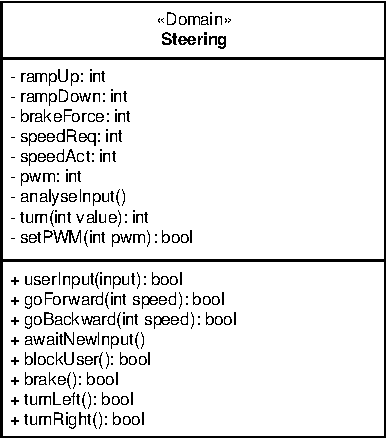
\includegraphics[]{../fig/diagrammer/bil/cd_steering.pdf}
\caption{Klassebeskrivelse af boundary-klassen Steering}
\label{fig:cd_Steering}
\end{figure}

\textbf{Attributter}

\begin{table}[H]
\begin{tabularx}{\textwidth}{| l | l | Z |} \hline
Navn & Type & Beskrivelse \\\hline
\texttt{motorPWMOutValue\_} & \texttt{int} &Variabel der indeholder værdien den skal sendes til PWM hardware på Pi \\\hline
\texttt{direction\_} & \texttt{bool} &Variabel der indeholder værdien om bilen skal kører frem eller tilbage.\\\hline
\texttt{minServoPWM\_} & \texttt{int} &Minimum værdi for softwarePWM.\\\hline
\texttt{maxServoPWM\_} & \texttt{int} &Maximum værdi for softwarePWM.\\\hline
\texttt{dataClassPtr\_} & \texttt{Data*} &En pointer til det objekt af typen Data der ønskes læst og skrevet data til.\\\hline
\texttt{SettingsPtr\_} & \texttt{Settings*} &En pointer til det objekt af typen Settings der ønskes skrevet data til.\\\hline
\texttt{logPtr\_} & \texttt{Log*} &En pointer til et object af typen Log. Gør det muligt at kalde funktioner fra Log objektet.\\\hline
\texttt{dState\_} & \texttt{double } &Gemmer sidste motorPWMOutValue værdi til næste udregning .\\\hline
\texttt{iState\_} & \texttt{double} &Gemmer error værdier til udregning af integral ledet i PID regulering.\\\hline
\texttt{iMax\_} & \texttt{double } &Max værdi af integral ledet.\\\hline
\texttt{iMin\_} & \texttt{double } &Min værdi af integral ledet.\\\hline
\texttt{iGain\_} & \texttt{double } &Integral gain.\\\hline
\texttt{pGain\_} & \texttt{double } &Proportional gain.\\\hline
\texttt{dGain\_} & \texttt{double } &Derivative gain.\\\hline
\texttt{error\_} & \texttt{double } &Fejl værdien mellem ønsket hastighed og aktuel hastighed.\\\hline
\texttt{pTemp\_} & \texttt{double } &Værdi for udregnet proportional værdi.\\\hline
\texttt{dTemp\_} & \texttt{double } &Værdi for udregnet derivative værdi.\\\hline
\texttt{iTemp\_} & \texttt{double } &Værdi for udregnet integral værdi.\\\hline


\end{tabularx}
\caption{Attributter for klassen Steering}
\label{table:attr_steering}
\end{table}

\newpage
\textbf{Metoder} 

%TODO fix position

\begin{table}[H]
\begin{tabularx}{\textwidth}{| L{2.5 cm} | Z |} \hline
Prototype & \texttt{int userInput(unsigned char speedForward, unsigned char speedBackward, 
	char turn, char brake)} \\\hline
Parametre & \texttt{speedForward} \newline Den ønskede hastighed fremad. 0..255\newline
		\texttt{speedBackward} \newline Den ønskede hastighed bagud. 0..255\newline
		\texttt{turn} \newline Den ønskede drejning på forhjul. -128..127\newline
		\texttt{brake} \newline Der skal bremses. 0..1\newline 
 \\\hline
Returværdi &  \texttt{int} \newline 1 hvis alle operationer er gået okay ellers -1. \\\hline
Beskrivelse & Metoden sørger for at opdaterer retning og hastighed på bilen. \\\hline
\end{tabularx}
\caption{Metodebeskrivelse for \texttt{userInput}}
\label{table:met_userInput}
\end{table}



\begin{table}[H]
	\begin{tabularx}{\textwidth}{| L{2.5 cm} | Z |} \hline
		Prototype & \texttt{void PWMUpdate( )} \\\hline
		Parametre &   
		\\\hline
		Returværdi &  \texttt{int} \newline 1 hvis alle operationer er gået okay ellers -1. \\\hline
		Beskrivelse & Metoden sørger for at opdaterer PWM output til hastighed på bilen. \\\hline
	\end{tabularx}
	\caption{Metodebeskrivelse for \texttt{PWMUpdate}}
	\label{table:met_PWMUpdate}
\end{table}

\begin{table}[H]
	\begin{tabularx}{\textwidth}{| L{2.5 cm} | Z |} \hline
		Prototype & \texttt{int brake( )} \\\hline
		Parametre & 
		\\\hline
		Returværdi &  \texttt{int} \newline 1 hvis alle operationer er gået okay ellers -1. \\\hline
		Beskrivelse & Metoden sørger for bremse på bilen ned i hastighed. \\\hline
	\end{tabularx}
	\caption{Metodebeskrivelse for \texttt{brake}}
	\label{table:met_brake}
\end{table}

\begin{table}[H]
	\begin{tabularx}{\textwidth}{| L{2.5 cm} | Z |} \hline
		Prototype & \texttt{int softbrake( )} \\\hline
		Parametre & 
		\\\hline
		Returværdi &  \texttt{int} \newline 1 hvis alle operationer er gået okay ellers -1. \\\hline
		Beskrivelse & Metoden sørger for at bilen løber hastighed af med 0 PWM output. \\\hline
	\end{tabularx}
	\caption{Metodebeskrivelse for \texttt{softbrake}}
	\label{table:met_softbrake}
\end{table}

\begin{table}[H]
	\begin{tabularx}{\textwidth}{| L{2.5 cm} | Z |} \hline
		Prototype & \texttt{int turn(signed char value)} \\\hline
		Parametre & \texttt{value} \newline
		Værdien for retning af bilen
		\\\hline
		Returværdi &  \texttt{int} \newline 1 hvis alle operationer er gået okay ellers -1. \\\hline
		Beskrivelse & Metoden sørger for at udregne retningen på bilens forhjul og sende værdien til software PWM output. \\\hline
	\end{tabularx}
	\caption{Metodebeskrivelse for \texttt{turn}}
	\label{table:met_turn}
\end{table}

\begin{table}[H]
	\begin{tabularx}{\textwidth}{| L{2.5 cm} | Z |} \hline
		Prototype & \texttt{int motorSetPWM(unsigned char speedForward, unsigned char speedBackward)} \\\hline
		Parametre & \texttt{speedForward} \newline Den ønskede hastighed fremad. 0..255\newline
		\texttt{speedBackward} \newline Den ønskede hastighed bagud. 0..255
		\\\hline
		Returværdi &  \texttt{int} \newline 1 hvis alle operationer er gået okay ellers -1. \\\hline
		Beskrivelse & Metoden sørger for at opdaterer retning frem/tilbage på bilen og bremse hvis bilen kører for stærkt til at vende retningen med det samme. \\\hline
	\end{tabularx}
	\caption{Metodebeskrivelse for \texttt{motorSetPWM}}
	\label{table:met_motorSetPWM}
\end{table}

